\documentclass[12pt,a4paper]{article}
\usepackage{datetime}
\usepackage{hyperref}
\usepackage{graphicx}
\usepackage{color}
\usepackage{amsmath}

\begin{document}

\title{BOLODSP Software User's Guide}

\author{Jack Lovell\thanks{\texttt{jack.lovell@durham.ac.uk}}}

\date{\today}

\maketitle

\abstract{This document serves as a guide for the end user to work with the BOLODSP software package which is bundled with D-TACQ's ACQ400 series firmware.
  A basic theory of operation is presented, and the parameters which control the operation of the BOLODSP module are discussed. General operation of
  D-TACQ's software, and the implementation details of the software and associated FPGA firmware module, are out of scope.}

\tableofcontents

\section{Introduction}
The BOLODSP software package is part of a custom module for D-TACQ ACQ400 series products used to operate the BOLO8BLF hardware module. It provides
software control of the BOLODSP FPGA module through a series of Linux commands, as well as some helper applications to simplify the fine tuning of the
signal processing capabilities of the module.

This document is \textit{not} a general user guide for D-TACQ software. For that, refer to the D-TACQ 4G user guide at \mbox{\url{http://www.d-tacq.com}}.
It is only concerned with the commands and settings provided by the package itself. Likewise, any requests for support with operating a system with this
package installed should be directed to D-TACQ directly, and not to the author, unless the query is specifically about an aspect of the BOLODSP module.

\section{Theory of Operation}
\subsection{Voltage Measurement}
\label{sec:voltage}
\begin{figure}
  \centering
  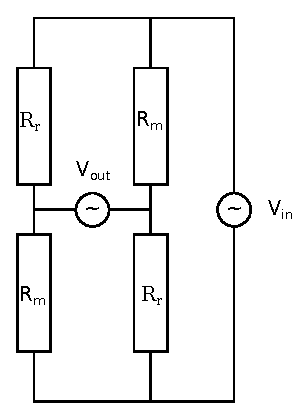
\includegraphics[width=0.3\textwidth]{sensor_schematic.eps}
  \caption{Electrical schematic of bolometer sensor\label{fig:sensor}}
\end{figure}
A resistive bolometer consists of 4 resistors in a Wheatstone bridge configuration (see Figure~\ref{fig:sensor}), as described in Ref~\cite{mast-1991}.
The two resistors marked $R_m$ are ``measurement'' resistors, which are in thermal contact with a thin foil. Incident radiation heats the foil and hence
the resistors, increasing their resistance. The two resistors marked $R_r$ are ``reference'' resistors: they are not in contact with the foil, and so their
temperature (and hence resistance) remain constant.

When a voltage $V_{in}$ is applied across one diagnoal of the bridge as shown, there will be zero output voltage $V_{out}$ if the bridge is balanced.
However, if the measurement resistors have increased resistance compared to the reference resistors, the bridge will be unbalanced, and $V_{out}$ will be
non-zero. By measuring $V_{out}$ it is therefore possible to calculate the resistance change of the foil, and by knowing the electrical and thermal
properties of the sensor it is possible to then infer the temperature change and the absorbed power. The details of these calculations are out of the
scope of this document.

To minimise noise in the system, AC synchronous detection is used to measure $V_{out}$. An AC excitation voltage $V_{in}$ is applied to the bridge,
typically a sinusoid with a frequency of a few 10s of kHz. The amplitude of $V_{out}$ at the same frequency is measured, and this voltage amplitude is
used in the bolometer equation to determine the absorbed power. The amplitude calculation (demodulation) is performed on the FPGA module, as follows.

The excitation voltage $V_{in}$ is of the form
\begin{equation}
  \label{equ:vin}
  V_{in} = V_0\sin(\omega t)
\end{equation}
Where $V_0$ is the amplitude of the excitation voltage and $\omega$ is the frequency. The output from the bridge due to the bridge imbalance is of the form:
\begin{equation}
  \label{equ:vout}
  V_{out} = A\sin(\omega t + \phi)
\end{equation}
Where the amplitude $A$ is the quantity we want to measure, and $\phi$ is the phase difference between the output and excitation voltages. This phase
shift is due to round trip time and parasitic capacitance in the system, and can be significant when there is a long cable between the electronics and
the sensor.

By multiplying $V_{out}$ with a normalised form of $V_{in}$ (which we shall call $V_{ref,i}$) and time averaging to remove the $2\omega$ frequency component
from the resulting signal, we can obtain the amplitude, assuming it varies slowly compared to the time averaging window. This is known as the ``in-phase''
component, since the signal is multiplied by a reference voltage of the same phase as the excitation voltage:
\begin{equation}
  \label{equ:I}
  \begin{split}
  I &= \frac{1}{n\pi}\int_{0}^{2n\pi}V_{ref,i}V_{out}\mathrm{d}\omega t \\
  &= \frac{1}{n\pi}\int_{0}^{2n\pi}\sin(\omega t) A \sin(\omega t + \phi)\mathrm{d}\omega t \\
  &= \frac{A}{2}\cos \phi
  \end{split}
\end{equation}
Equation~\ref{equ:I} still depends on the phase $\phi$. Traditionally, some phase shift has been applied to $V_{ref,i}$ such that $\phi = 0$ to remove the
phase dependence on $I$, but we employ a more general method. Consider a second reference, $V{ref,q}$ which is a quarter of a period out of phase with the
excitation voltage:
\begin{equation}
  \label{equ:Q}
  \begin{split}
  Q &= \frac{1}{n\pi}\int_{0}^{2n\pi}V_{ref,q}V_{out}\mathrm{d}\omega t \\
  &= \frac{1}{n\pi}\int_{0}^{2n\pi}\cos(\omega t) A \sin(\omega t + \phi)\mathrm{d}\omega t \\
  &= -\frac{A}{2}\sin \phi
  \end{split}
\end{equation}
We can now combine Equations~\ref{equ:I} and~\ref{equ:Q} to remove the phase dependence:
\begin{equation}
  \label{equ:A}
  A = 2\sqrt{I^2 + Q^2}
\end{equation}
Equation~\ref{equ:A} thus gives a measure of the amplitude of the output voltage independent of phase, and hence independent of the hardware used. This
method is known as ``quadrature detection''.

For completeness, the phase is given by:
\begin{equation}
  \label{equ:phi}
  \phi = -\tan^{-1}\left(\frac{Q}{I}\right)
\end{equation}

On the FPGA, the time averaging is done using a low-pass fiter. The choice of filter coefficients will affect the integration time, or alternatively the
bandwidth of the output. Higher bandwidth allows higher time resolution, but comes at the cost of increased noise in the measurement, since higher
frequency noise components are less suppressed. A helper script exists to calculate the appropriate filter coefficients for a given bandwidth, and load
them onto the FPGA (see Section~\ref{sec:lpfdesign}).

\subsection{Voltage Offset}
\label{sec:offset}
No sensor is perfect, in the sense that the bridge will never be perfectly balanced in the absense of any input power. Likewise, no electronics is perfect,
and there will always be some cross talk between excitation and measurement voltages. This leads to a voltage offset with no input power:
\begin{equation}
  \label{equ:voff}
  V_{off} = A_{off}e^{i\phi_{off}}
\end{equation}
Note that the offset voltage has both an amplitude \textit{and} phase, which may be different to the phase of the signal due to incident power, making the
measured voltage a complex signal. It is necessary to subtract this offset from the measured signal using a suitable complex subtraction, either by
decomposing into real ($I$) and imaginary ($Q$) parts and subtracting the real and imaginary parts respectively of the offset, or by performing a
vector-based subtraction using the cosine rule.

The FPGA firmware has the capability to perform the first of these methods on-chip, using user-loadable offset values for each channel. When offset
subtraction has been correctly performed, the remaining phase should be constant (being only a property of the geometry), and the remaining amplitude will
be a measure only of the bridge imbalance (and hence the temperature change of the sensor foil). The phase is therefore a useful measurement for data
validation.

\subsection{Real-Time Power Output}
\label{sec:rtpower}
The physics involved in calculating the power absorted by the foil from the resistance change of the meander resistors is complex, particularly when an AC
excitation voltage is involved. For a throrough treatment of the subject, see Ref~\cite{giannone-2002}. However, the following simplified formula gives a
good approximation of the more complex result:
\begin{equation}
  \label{equ:pbol}
  P = \frac{1}{S}\left(A + \tau \frac{\mathrm{d}A}{\mathrm{d}t}\right)
\end{equation}
Here, $S$ is the sensitivity of the sensor, and $\tau$ is the cooling time. Both these values can be calculated using an in-situ calibration proceduce, as
described in Section~\ref{sec:calibration}.

The flexibility of the FPGA's digital filtering means it is possible to design a filter to both perform the time averaging described in
Section~\ref{sec:voltage}, and adding to this the time derivative as in Equation~\ref{equ:pbol}. Using this filter (known as a ``deconvolution'' filter)
will produce an estimate of the incident power straight from the bridge voltage measurement, with a latency of about 1ms, which should be quick enough to
use in a real-time control loop. The design of this filter requires an accurate calibration, and is discussed in Section~\ref{sec:calibration}.

\subsection{Calibration}
\label{sec:calibration}
It can be seen from Equation~\ref{equ:pbol} that at least 2 quantities need to be determined from a calibration: the sensitivity $S$ and the cooling time
$\tau$. The sensitivity can be determined by measuring the rise in the voltage output for a known input power, and the cooling time can be calculated by
fitting an exponential decay to the voltage curve as the sensor cools immediately after removing all input power. In the BOLO system, the input power is
provided by ohmic heating, by applying a DC bias to both $V_{in}$ and $V_{out}$, whilst at the same time keeping the AC excitation voltage of $V_{in}$ to
simulate operation with radiation heating as closely as possible.

\begin{figure}
  \centering
  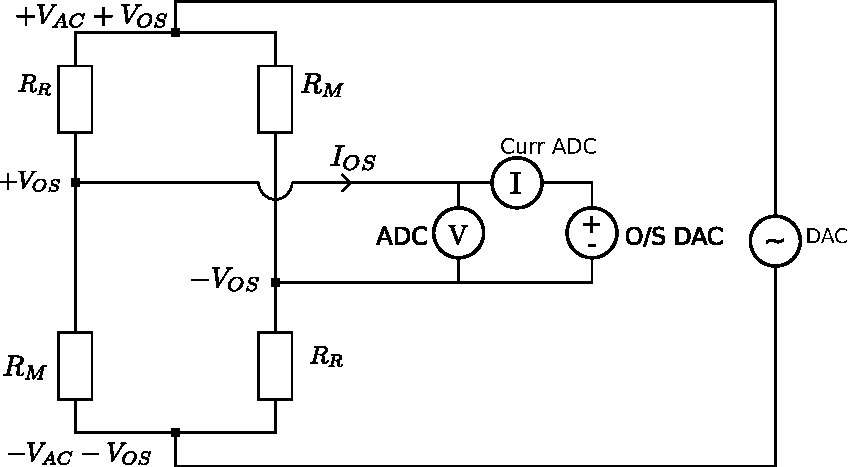
\includegraphics[width=0.5\textwidth]{calibration.eps}
  \caption{Electrical schematic of the calibration procedure\label{fig:calibration}}
\end{figure}

The calibration producure is described in some detail in~\cite{lovell-2015}. Figure~\ref{fig:calibration}, taken from that paper, shows the calibration
proceedure. The application of $V_{OS}$ is such that current flows through the two measurement resistors $R_M$, but not through the reference resistors
$R_R$. This causes only the measurement resistors to be ohmically heated, with a heating power given by
\begin{equation}
  \label{equ:pohmic}
  P_{OH} = 2 V_{OS} I_{OS}
\end{equation}
When the ohmic heating is switched off, the sensor cools. The bridge voltage (amplitude and phase) measured during cooling provides a number of useful
calibration values. They must however be converted into Carteisan representation ($I$ and $Q$) first:
\begin{itemize}
\item{The offsets $A_{off}$ and $\phi_{off}$ can be calculated using Equations~\ref{equ:I} and~\ref{equ:Q}, using $I_{off} = I(t\rightarrow\infty)$ and $Q_{off}
    = Q(t\rightarrow\infty)$}
\item{The cooling time can be calculated by fitting an exponential decay of the $I$ and $Q$ cooling curves. The decay time constant is the cooling time.
    It should be the same (to within errors) for both curves.}
\item{The sensitivity is given by $S = \frac{P_{OH}}{\Delta A}$, where $P_{OH}$ is given by Equation~\ref{equ:pohmic} and $\Delta A$ is given by
    Equation~\ref{equ:A}, using $\Delta I = I(t=0) - I_{off}$, and $\Delta Q = Q(t=0) - Q_{off}$.}
\end{itemize}
During the calibration, the FPGA measures $V_{OH} = 2V_{OS}$ and $I_{OS}$, in addition to $A$ and $\phi$, thus providing all the required data for a
calibration in one place. Note the difference between $V_{OH}$ and $V_{OS}$: the latter is provided only for illustration, whereas the former is what is
configured by software and subsequently measured.

\section{Data Outputs}
\label{sec:outputs}
\subsection{Output Channel Format}
\label{sec:channels}
For each physical channel on a BOLO8, there are 3 ``logical'' output channels. This means each BOLO8 site has 24 output channels, each of which can be read
like any other D-TACQ output (see the D-TACQ 4G user guide for details). All channels are 4-byte signed integers. The channels are arranged as follows:
\begin{enumerate}
\item{The voltage amplitude $A$ from the quadrature synchronous detection process (Section~\ref{sec:voltage}).}
\item{The phase $\phi$ from the quadrature synchronous detection process (Section~\ref{sec:voltage}).}
\item{The third channel depends on the operating mode:}
  \begin{enumerate}
  \item{During normal mode: the real-time power calculation from the deconvolution process (Section~\ref{sec:rtpower}).}
  \item{During calibration mode: a combination of the ohmic heating voltage $V_{OH}$ and current $I_{OH}$ (Section~\ref{sec:calibration}). The top 2 bytes of
      each 4-byte sample are the voltage, and the bottom 2 bytes are the current. In other words, this output is $V_{OH} \times 2^{16} + I_{OH}$. In this
      scenario, $V_{OH}$ is a signed 2-byte integer, and $I_{OH}$ is an unsigned 2-byte integer.}
  \end{enumerate}
\end{enumerate}

For a phycial channel $N$ (numbered 1--8 per site), logical channel $3N-2$ is the voltage amplitude, $3N-1$ is the voltage phase and $3N$ is either the
real-time power or calibration quantities. So for example, for physical channel 3, logical channel 7 is the amplitude, 8 is the phase and 9 is
power/calibration signals.

\subsection{Data Scaling}
\label{sec:scaling}
The following are the numerical conversion factors to convert from raw counts (the 2- or 4-byte values read from the device) into physical units. There is
a dependence on $V_{gain}$, which is the voltage gain used on the BOLO8's ADCs. The value can be read back as a knob in CSS or EPICS (or your favourite data
acquisition tool); contact D-TACQ for the details of setting and reading these values. The recommended gain is 1V2 (1.25V), since the bolometer signals are
typically small (10s to a few 100s of mV), even with strong radiation.

There is also a dependence on the CORDIC scale factor:
\begin{equation}
  \label{equ:cordic}
  \begin{split}
    Z_{30} &= \prod_{i=1}^{30}\sqrt{1 + 2^{-2i}} \\
    &= 1.1644353\ldots
  \end{split}
\end{equation}
This is due to the algorithm used to convert $I$ and $Q$ into $A$ and $\phi$ on the FPGA\@.

The scalings are as follows:
\begin{equation}
  \label{equ:avolts}
  \begin{split}
    A(V) &= A(counts) V_{gain} \frac{20}{18 \times 2^{24} \times Z_{30}} \\
    &= A(counts) V_{gain} \times 5.6875105\ldots \times 10^{-8}
  \end{split}
\end{equation}

\begin{equation}
  \label{equ:phirad}
  \begin{split}
    \phi(rad) &= \phi(counts) \times 2^{-29} \\
    &= \phi(counts) \times 1.8626451\ldots \times 10^{-9}
  \end{split}
\end{equation}

\begin{equation}
  \label{equ:pwatts}
  \begin{split}
    P(W) &= P(counts) V_{gain} \frac{20}{18 \times 2^{24} \times Z_{30}} \\
    &= P(counts) V_{gain} \times 3.6400067\ldots \times 10^{-6}
  \end{split}
\end{equation}

\begin{equation}
  \label{equ:vdcvolts}
  \begin{split}
    V_{OH}(V) &= V_{OH}(counts) V_{gain} \times 2^{-15} \\
    &= V_{OH} V_{gain} \times 3.0517578\ldots \times 10^{-5}
  \end{split}
\end{equation}

\begin{equation}
  \label{equ:curramps}
  \begin{split}
    I_{OH}(A) &= I_{OH}(counts) \times \frac{25}{3 \times 2^{12} \times 1000} - I_{off} \\
    &= I_{OH}(counts) \times 2.0345052\ldots \times 10^{-6} - I_{off}
  \end{split}
\end{equation}

$I_{off}$ in Equation~\ref{equ:curramps} is the current reading when $V_{OH} = 0$, i.e.\ no bias voltage is applied. In theory it should be around
$20.83 \times 10^{-3} \mathrm{A}$ but will vary slighly between channels. The most reliable way to measure $I_{off}$ is to take the mean value of
the current during the cooling part of the calibration.

\section{Control Knobs}
\label{sec:knobs}
This section describes the control knobs available for the BOLODSP module. They are read and set in the same way as standard D-TACQ knobs using the remote
command interface. See the D-TACQ 4G user guide for details.

\subsection{Low-level knobs}
\label{sec:knobsll}
These control knobs are a fairly low level interface to the underlying FPGA module. For the most part they will be set by utility scripts. The ones which
may require the user to manually set them (or at least write a script to do so during the shot cycle) are documented here.

\subsubsection{DSP{\textunderscore}RESET}
Set to 1 to reset the BOLODSP firmware module. Set to 0 to remove from reset. To ensure correct channel ordering and an accurate time base for the data,
the module should be reset before each acquisition (transient or streaming). This is automatically handled by the calibration script.

\subsubsection{STEP{\textunderscore}SIZE}
This is used to generate the AC excitation voltage to the sensor. The excitation voltage is a sine wave of 18V amplitude. Note that the electronics is
capable of $\pm 20\mathrm{V}$ output; the 2V headroom is left to enable DC biasing during calibration. Due to implementation details in the BOLODSP
module, the STEP{\textunderscore}SIZE value $S$ required to produce an excitation voltage of $f$ Hz is given by:
\begin{equation}
  \label{equ:step_size}
  S = \frac{f}{f_{clk}} \times 2^{27}
\end{equation}
Here, $f_{clk}$ is the system clock frequency. Is is typically 100 MHz on older D-TACQ systems, and 125 MHz on newer systems. Contact D-TACQ if you are
unsure which frequency to use (or pick one and check the output on a scope to see if it's the correct frequency).

There also exists a script, \path{/usr/local/bin/set.fdrive}~\texttt{<freq>}, which takes a frequency in Hz and automatically sets the register
correctly. It can be executed by SSHing into the unit. By default it assumes 100 MHz system clock, but this can be changed by modifying the script
contents (contact D-TACQ or the author for details).

\subsubsection{Calibration}
Set to 1 to put the device in calibration mode, 0 to put it in normal mode. This changes the data output in the third logical channel for each physical
channel (Section~\ref{sec:channels}). Again, this is done automatically by the calibration script.

\subsection{High-level knobs}
\label{sec:knobshl}
These control knobs interface with the BOLODSP module at a higher level. Their inputs are in physical units, rather than register settings, and the
utility scripts read these knobs in order to set the lower-level knobs. All high-level knobs presented by the BOLODSP package are described here, and
should be set by the user.

\subsubsection{DIODE{\_}DROP{\_}V}
This value, in volts, sets the extra voltage to apply to one diagonal of the bridge to compensate for the voltage drop across diodes in the electronics.

The electronics features some diodes for noise reduction. There will be a voltage drop across these diodes, meaning that the applied bias voltage $V_{OH}$
in calibration will be less than the requested voltage on one of the bridge diagonals. Set this knob (in volts) to apply an extra voltage across that
diagonal to compensate for the voltage drop. The value should be tweaked until the measured ohmic heating voltage $V_{OH}$ (Section~\ref{sec:channels}) is
close to that set by the VBIAS knob. As a guide, when VBIAS is set to 1V, the diode voltage drop is about 0.5V.

\subsubsection{FILTER{\_}BANDWIDTH}
As mentioned in Section~\ref{sec:voltage}, the choice of filter affects the trade-off between noise levels and time resolution. The filters themselves are
designed using helper scripts (Section~\ref{sec:lpfdesign}). Those scripts take the value of this knob to design a filter with a given bandwidth. The
bandwidth should be specified in Hz.

\subsubsection{THEAT}
This value, in seconds, specifies the length of time spent ohmically heating the sensor during calibration. It should be long enough to ensure the sensor
has reached equilibrium, i.e.\~several cooling times.

\subsubsection{TCOOL}
This value, in seconds, specifies the length of time to continue measuring the calibration curve after ohmic heating is turned off. It thus controls the
amount of the cooling curve measured. Like with THEAT, it should be set to multiple cooling times such that the sensor is nearly back in thermal
equilibrium at the end of the measurement.

\subsubsection{VBIAS}
This value, in volts, specifies the bias voltage $V_{OH}$ to be used to ohmically heat the bridge during calibration. It must be $<1.2\mathrm{V}$. The
required setting for DIODE{\_}DROP will typically depend upon this knob.

\subsubsection{CAL{\_}EN}
Set this to 1 to enable a calibration before a shot. You should ensure that the data acquisition system of which the unit is a part is set up to run 2
acquitisions during the shot cycle: one to acquire the calibration data and a second to acquire the shot data.

This knob is ignored by the BOLODSP module and software, but may be helpful for user-written shot-cycle scripts to examine and work out what they need to
do.

\subsubsection{CAL{\_}DELAY}
This value, in seconds, specifies the length of time to wait between the start of a shot cycle (i.e.~prepare/arm) and the start of a calibration
procedure. It allows the user to cause the calibration procedure to run at a known time in the shot initialisation sequence. This could for example mean
performing the calibration as close as possible to the start of the shot, for conditions as similar as possible during the calibration and shot, or
performing the calibration earlier before sources of electrical noise such as coil power supplies are switched on.

Like the CAL{\_}EN knob, this is ignored by the BOLODSP module and software, but exists to allow user-written shot-cycle scripts to examine and work out
what they need to do.

\bibliographystyle{ieeetr}
\bibliography{refs}


\end{document}
